\section{Distribuição Gaussiana}

\subsection{O que é a Distribuição Gaussiana?}
A \textbf{distribuição Gaussiana} ou \textbf{distribuição normal} é uma das distribuições mais importantes em razão da sua enorme presença nos mais variados campos do conhecimento. Se trata de uma curva de distribuição simétrica em torno do seu ponto médio. Ela possui a peculiaridade de ter a média, mediana e moda dos dados com o mesmo valor.

\subsection{Variável aleatória]}
\textbf{Variável aleatória} é um valor retirado de uma distribuição estatística e que não possui um valor fixo. O seu valor depende de fatores aleatórios. Ex: o resultado do lançamento de um dado pode dar qualquer número entre 1 e 6.

Uma variável aleatória que pode assumir apenas um número finito ou uma sequência infinita enumerável de valores é considerada \textbf{discreta}. Aquele que pode assumir qualquer valor no intervalo dos números reais é considerado \textbf{contínuo}. 

Uma \textbf{variável aleatória contínua} é uma variável aleatória que pode tomar qualquer valor numérico em um determinado intervalo ou coleção de intervalos (geralmente do conjunto dos números reais). Ex: uma variável aleatória que mede o tempo que leva para algo ser feito é contínua, pois ela pode assumir infinitos valores.

Como existe um número infinito de valores em qualquer intervalo, não faz sentido falar sobre a probabilidade da variável aleatória assumir um valor específico. Em vez disso, é considerada a probabilidade de uma variável aleatória contínua estar dentro de um determinado intervalo. É a chamada \textbf{Função Densidade de Probabilidade}.

\subsection{Função Densidade de Probabilidade}

É a função $f(x)$  de uma variável aleatória contínua cuja integral em um intervalo dá a probabilidade de que o valor da variável esteja dentro desse mesmo intervalo. Ou seja, \textbf{densidade de probabilidade} não é probabilidade. Somente quando a função for integrada entre dois limites é que ela produzirá uma probabilidade, sendo equivalente à área sob a curva da função densidade de probabilidade entre esses dois limites:

\[\large \int_{a}^{b} f(x)dx = P(a\leq x\leq b)\]

As funções densidade de probabilidade devem sempre obedecer à esses 2 requisitos:
\begin{itemize}
\item $f(x)$ deve ser não negativo para cada valor da variável aleatória: $f(x) > 0$
\item A área total sob a curva de probabilidade vale sempre 1: $\int_{-\infty }^{\infty} f(x)dx = 1$
\end{itemize}

A forma da função de densidade de probabilidade em todo o seu domínio é chamada de \textbf{distribuição de probabilidade}. A distribuição de probabilidade mais importante é a chamada \textbf{distribuição normal}, também chamado de \textbf{curva em forma de sino} devido à sua forma característica.

\subsection{Distribuição Normal ou Gassiana}

A distribuição normal é a distribuição de probabilidade mais importante no estudo da estatística devido à sua presença em muitos fenômenos naturais, por exemplo: a altura das pessoas, pressão arterial, erro de medição e pontuações de QI seguem a distribuição normal.

Como já foi dito, a probabilidade de uma observação assumir um valor entre dois pontos quaisquer é igual à área sob a curva da densidade de probabilidade compreendida entre esses dois pontos. No caso de uma curva de distribuição normal teórica, a regra é: 

\begin{itemize} 

\item $68,26\%$ da população ou amostra está dentro de uma região que varia de $\mu \pm \sigma$ 
\item $95,44\%$ da população ou amostra está dentro de uma região que varia de $\mu \pm 2\sigma$
\item $99,72\%$ da população ou amostra está dentro de uma região que varia de $\mu \pm 3\sigma$
\item $99,99\%$ da população ou amostra está dentro de uma região que varia de $\mu \pm 4\sigma$ 

\end{itemize}

\begin{figure}[H]
	\centering
	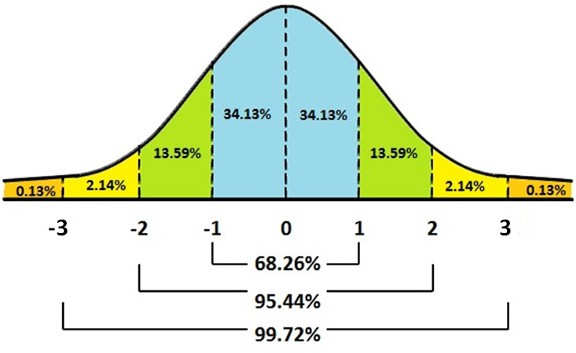
\includegraphics[width=1\textwidth]{./Imagens/Distribuição Normal/GA1.png} 
	\caption{Distribuição normal}
	\label{fig:GA1}
\end{figure}

\subsection{Densidade para a distribuição normal}
Uma variável aleatória contínua X tem distribuição normal se sua função densidade de probabilidade for dada por:

\[ \large p(x) = \frac{1}{\sigma \sqrt{2 \pi  }}e^{-\frac{1}{2} (\frac{x-\mu}{\sigma})^2} \]

Onde $\sigma$ é o \textbf{desvio padrão} da distribuição e $\mu$ é a \textbf{média}.

\subsection{Desvio padrão}

Comumente representado pelo símbolo $\sigma$, é uma medida de dispersão em torno da média populacional ou amostral de uma variável aleatória. Quanto maior o seu valor maior a ampla de valores na qual os dados estão espalhados. Um baixo desvio padrão indica que os pontos dos dados tendem a estar próximos da média.

\subsection{Fórmula para o desvio padrão}

O desvio padrão populacional ou amostral é a raiz quadrada da variância populacional ou amostral correspondente. 

\begin{itemize}

\item Quando o conjunto de dados é a população:

\[ \large \sigma = \sqrt{\frac{1}{N}\sum_{i=1}^{N}(x_{i}-\mu )^2} \]

\item Quando o conjunto de dados é uma amostra:

\[ \large \sigma = \sqrt{\frac{1}{N-1}\sum_{i=1}^{N}(x_{i}-\mu )^2} \]

\end{itemize}

\subsection{Distribuição Normal no Python}

Vamos traçar a curva de uma \textbf{distribuição normal padronizada}, que é uma curva normal de média $\mu = 0$ e desvio padrão $\sigma = 1$.

\begin{minted}{python}
	
from scipy.stats import norm
import matplotlib.pyplot as plt
import numpy as np 

fig, ax = plt.subplots(figsize = (8,5))

# definindo o domínio
dom = np.linspace(-2,2,1000)

plt.plot(dom, norm.pdf(dom, loc = 0 , scale = 1))
plt.title("Distribuição Normal Padronizada")
plt.xlabel("Valor")
plt.ylabel("Densidade")
ax.grid(True)
plt.show()

\end{minted}

\begin{figure}[H]
	\centering
	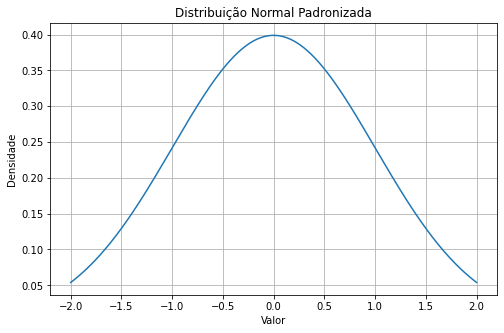
\includegraphics[width=1\textwidth]{./Imagens/Distribuição Normal/GA2.png} 
	\caption{Curva normal}
	\label{fig:GA2}
\end{figure}

Podemos alterar a forma da curva em sino alterando a média e o seu desvio padrão. Alterar a média deslocará a curva em direção a esse valor, isso significa que podemos alterar a posição da curva alterando o valor médio sem afetar a forma da curva.

\begin{minted}{python}
	
fig, ax = plt.subplots(figsize = (8,5))

x = np.linspace(-10,15,100)

medias = [0.0, 2.0, 5.0, 10.0]

for medias in medias:
ax.plot(x, norm.pdf(x,loc=medias), label=f"Médias: {medias}")

ax.set_xlabel('x')
ax.set_ylabel('pdf(x)')
ax.set_title('Distribuição Normal')
ax.legend(loc='best', frameon=True)
ax.set_ylim(0,0.45)
ax.grid(True)
	
\end{minted}

\begin{figure}[H]
	\centering
	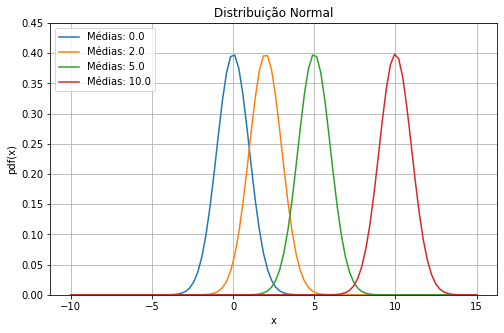
\includegraphics[width=1\textwidth]{./Imagens/Distribuição Normal/GA3.png} 
	\caption{Alterando a média}
	\label{fig:GA3}
\end{figure}

A forma da curva pode ser controlada pelo valor do desvio padrão. Um desvio padrão menor resultará em uma curva estreitamente limitada, enquanto um valor alto resultará em uma curva mais espalhada. 

\begin{minted}{python}
	
fig, ax = plt.subplots(figsize = (8,5))

x = np.linspace(-10,10,100)

stdvs = [1.0, 2.0, 3.0, 4.0]

for s in stdvs:
ax.plot(x, norm.pdf(x, scale=s), label=f'desvio padrão = {s}')

ax.set_xlabel('x')
ax.set_ylabel('pdf(x)')
ax.set_title('Distribuição Normal')
ax.legend(loc='best', frameon=True)
ax.set_ylim(0,0.45)
ax.grid(True)
	
\end{minted}

\begin{figure}[H]
	\centering
	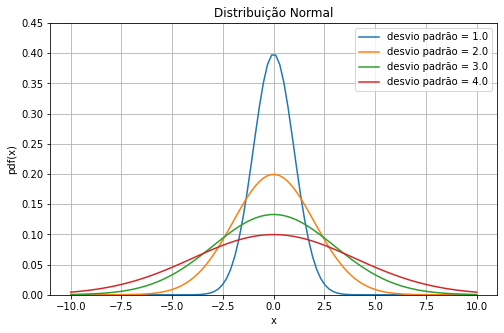
\includegraphics[width=1\textwidth]{./Imagens/Distribuição Normal/GA4.png} 
	\caption{Alterando o desvio padrão}
	\label{fig:GA4}
\end{figure}

\subsection{Função distribuição acumulada}

É a função $F(x)$ que indica a probabilidade de um determinado valor de uma variável aleatória X ser menor ou igual à x. Em termos matemáticos:

\[\large F(x) = P(X \leq x) = \int_{-\infty }^{x}f(x_{i})dx\]

\subsubsection{Calculando a probabilidade de ocorrência de dados específicos}

Vamos utilizar o conceito de função distribuição acumulada (CDF) e calcular a probabilidade de um valor estar abaixo de -1 ao escolhermos um valor aleatório da distribuição. Essa probabilidade será a área da região apresentada abaixo e terá um valor de aproximadamente $15,87\%$.

\begin{figure}[H]
	\centering
	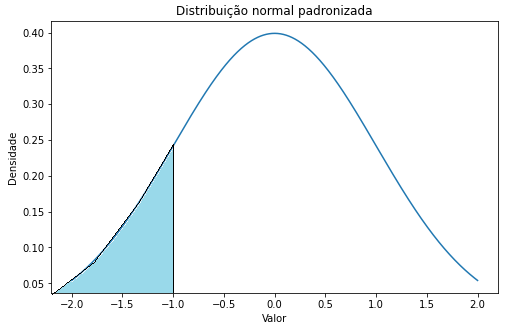
\includegraphics[width=1\textwidth]{./Imagens/Distribuição Normal/GA5.png} 
	\caption{Abaixo de -1}
	\label{fig:GA5}
\end{figure}

\begin{minted}{python}
prob = norm(loc = 0 , scale = 1).cdf(-1)
print(f"Probabilidade: {prob*100:.2f}%")
# Probabilidade: 15.87%
\end{minted}

Para calcular a probabilidade do valor estar entre uma região específica (entre 2 e 1 por exemplo):

\begin{figure}[H]
	\centering
	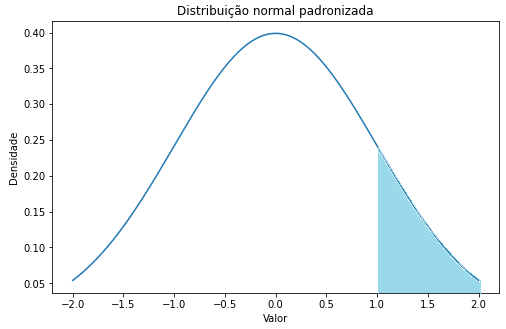
\includegraphics[width=1\textwidth]{./Imagens/Distribuição Normal/GA6.png} 
	\caption{Entre 1 e 2}
	\label{fig:GA6}
\end{figure}

\begin{minted}{python}
cdf_limite_superior = norm(loc = 0 , scale = 1).cdf(2)
cdf_limite_inferior = norm(loc = 0 , scale = 1).cdf(1)

prob = cdf_limite_superior - cdf_limite_inferior
print(f"Probabilidade: {prob*100:.2f}%")
# Probabilidade: 13.59%
\end{minted}

Para calcular a probabilidade do valor ser maior que x (0.5 por exemplo): 

\begin{figure}[H]
	\centering
	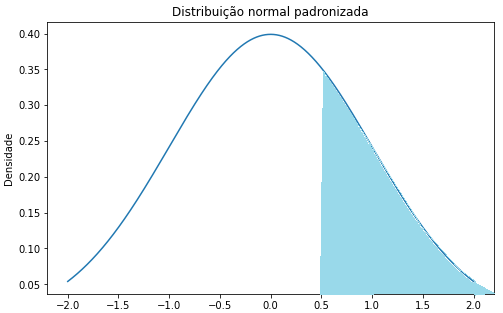
\includegraphics[width=1\textwidth]{./Imagens/Distribuição Normal/GA7.png} 
	\caption{Maior que 0.5}
	\label{fig:GA7}
\end{figure}

\begin{minted}{python}
prob = 1 - norm(loc = 0 , scale = 1).cdf(0.5)
print(f"Probabilidade: {prob*100:.2f}%")
# Probabilidade: 30.85%
\end{minted}

\subsection{Aplicações da Distribuição Normal}
\begin{itemize}
\item O matemático francês Abraham de Moivre, em seu Doctrine of Chances (1718), primeiro observou que as probabilidades associadas a variáveis aleatórias geradas discretamente (como as obtidas jogando uma moeda ou jogando um dado) podem ser aproximadas pela área sob o gráfico de uma função exponencial. Este resultado foi estendido e generalizado pelo cientista francês Pierre-Simon Laplace.
\item Em 1860, Maxwell supôes que a velocidade das colisões das partículas obedecem a distribuição normal.
\item Pode ser utilizado na análise da resistência dos materiais, onde os dados coletados podem ser generalizados para uma distribuição normal de forma a facilitar as simulações computacionais e torná-los mais práticos. 
\item Em projetos de engenharia no campo da ergonomia.
\end{itemize}